%%%%%%%%%%%%%%%%%%%%%%%%%%%%%%%%%%%%%%%%%%%%%%%%%%%%%%%%%%%%%%%%%%%%%%%%%%%

\documentclass{standalone}

\usepackage{amsmath}
\usepackage{mathptmx}
\usepackage{pgfplots}
\usetikzlibrary{external}
\tikzexternalize{interest}
\pgfplotsset{compat=1.15}

%% IEEE uses Times Roman font, so we'll default to Times.
%% These three commands make up the entire times.sty package.
\renewcommand{\rmdefault}{ptm}
\renewcommand{\ttdefault}{pcr}
\normalfont\selectfont

\begin{document}

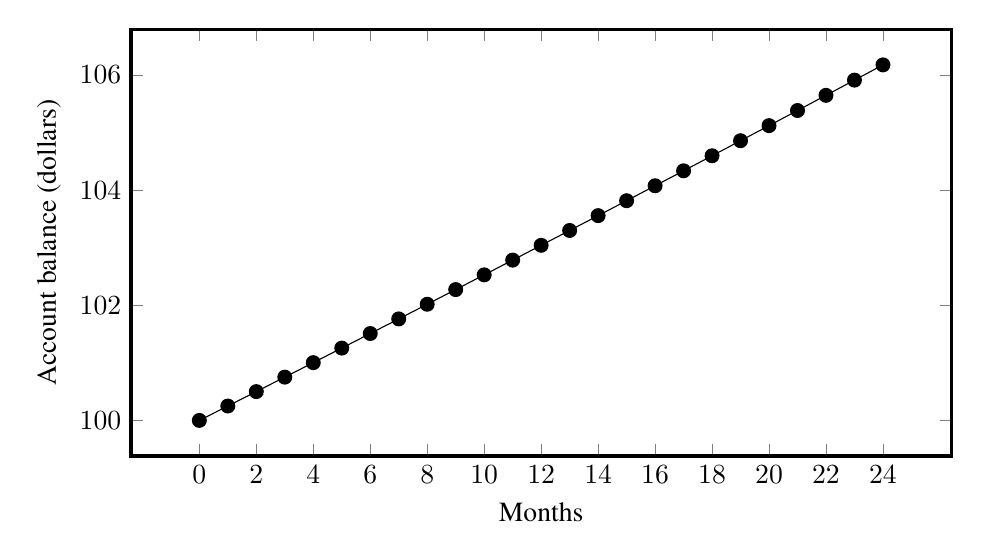
\begin{tikzpicture}
\tikzset{%%
  every mark/.append style={scale=1.0},%%
  scale=1.0%%
}
\pgfplotsset{%%
  every axis/.append style={font=\normalsize}%%
}
%%
\begin{axis}[%%
  axis line style=very thick,%%
  dotStyle/.style={mark size=2.5,black,mark color=black,mark=*},%%
  enlargelimits=true,%%
  height=7cm,%%
  plotStyle/.style={%%
    domain=4:17,%%
    mark=none,%%
    smooth,%%
    thick%%
  },%%
  width=12cm,%%
  %% x axis
  xlabel={\normalsize Months},%%
  xtick={0,2,4,6,8,10,12,14,16,18,20,22,24},%%
  xticklabels={$0$,$2$,$4$,$6$,$8$,$10$,$12$,$14$,$16$,$18$,$20$,$22$,$24$},%%
  %% y axis
  ylabel={\normalsize Account balance~(dollars)},%%
  scaled y ticks=false,%%
  y tick label style=/pgf/number format/fixed%%
]
%%
%%
\addplot[dotStyle] coordinates {
  (0, 100.000000)
  (1, 100.250000)
  (2, 100.500625)
  (3, 100.751877)
  (4, 101.003756)
  (5, 101.256266)
  (6, 101.509406)
  (7, 101.763180)
  (8, 102.017588)
  (9, 102.272632)
  (10, 102.528313)
  (11, 102.784634)
  (12, 103.041596)
  (13, 103.299200)
  (14, 103.557448)
  (15, 103.816341)
  (16, 104.075882)
  (17, 104.336072)
  (18, 104.596912)
  (19, 104.858404)
  (20, 105.120550)
  (21, 105.383352)
  (22, 105.646810)
  (23, 105.910927)
  (24, 106.175704)
};
\end{axis}
\end{tikzpicture}

\end{document}
